\section{Interface}

Nesta seção, descrevemos os elementos de interação entre o jogador e o
jogo.

\subsection{HUD}

A tela do jogador terá as informações a seguir, seguindo o modelo da
Figura \ref{fig:hud}
\begin{figure}[!ht]
 \centering
 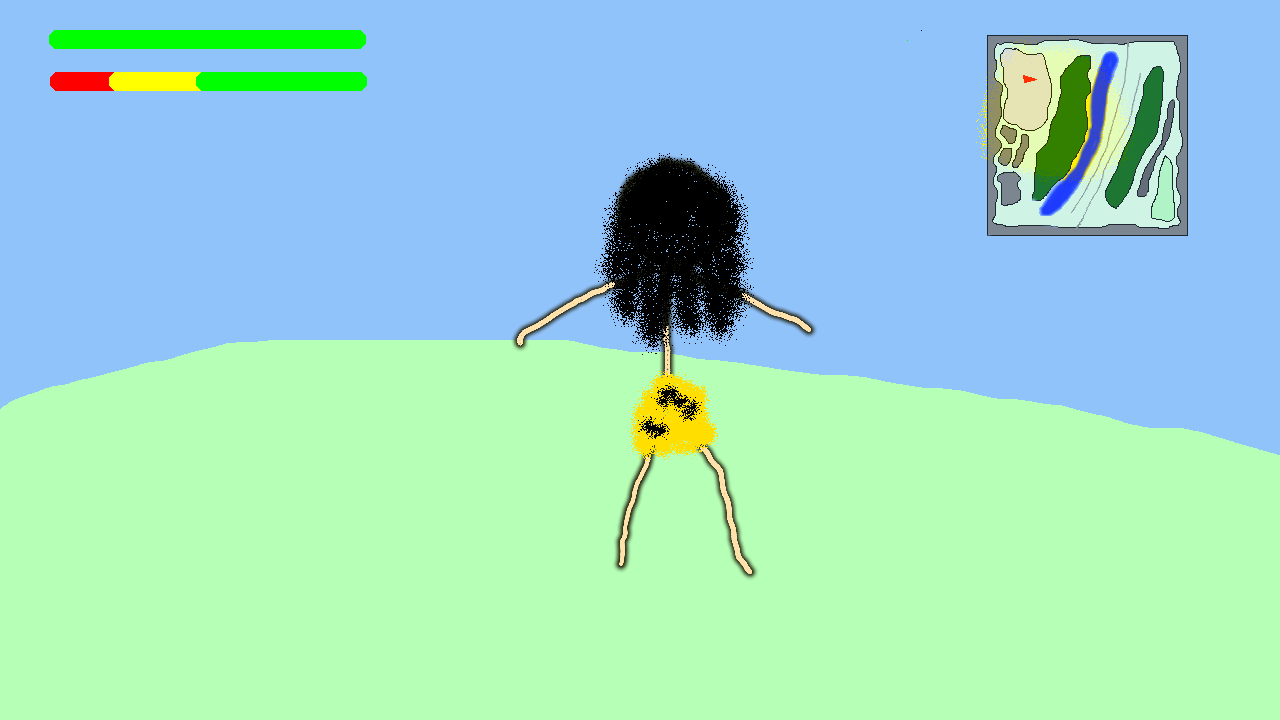
\includegraphics[scale=0.39]{hud.png}
 \caption{HUD}
 \label{fig:hud}
\end{figure}
\begin{enumerate}
 \item {\bf Barra de Vida:} Canto superior esquerdo da tela, no 
formato de uma barra horizontal. 
 \item {\bf Barra de Energia/Temperatura:} Quando houver esta barra,
ela estará no canto superior esquerdo da tela,
abaixo da barra de vida.
 \item {\bf Minimapa:} Canto superior direito, em forma de quadrado.
Será fixo e semi-transparente. Mostrará um esboço do mapa e um triângulo
indicando a posição e direção de Medrash. Existirá apenas na primeira fase.
\end{enumerate}

\subsection{Menus}

O jogo terá apenas dois menus. Um deles será o menu principal do jogo, e o 
outro será o menu de pausa.

\subsubsection{Menu Principal}

O menu principal terá as seguintes opções:
\begin{itemize}
 \item {\bf Começar novo jogo:} Apaga todas informações sobre o jogo atual,
se houver, e inicia um novo jogo.
 \item {\bf Continuar jogo:} Se houver um jogo em progresso, permite que
o usuário continue o mesmo. Caso contrário, esta opção estará desativada.
 \item {\bf Sair do jogo:} Sai do jogo, finalizando o software.
\end{itemize}

\subsubsection{Menu de Pausa}
O menu de pausa só pode ser acessado durante o jogo, e contém as seguintes
opções:
\begin{itemize}
 \item {\bf Continuar o jogo:} Sai do menu de pausa.
 \item {\bf Voltar ao menu principal:} Sai do jogo e volta ao menu 
principal. Não salva o jogo.
 \item {\bf Sair do jogo:} Sai do jogo e finaliza o software.
\end{itemize}

